%\documentclass[%
%reprint,
%%singlecolumn,
%superscriptaddress,
%%groupedaddress,
%%unsortedaddress,
%%runinaddress,
%%frontmatterverbose, 
%%preprint,
%%showpacs,preprintnumbers,
%%nofootinbib,
%%nobibnotes,
%%bibnotes,
%%pre, 
%floatfix,
%amsmath,
%amssymb,
%aps,
%notitlepage
%]{revtex4-1}
\documentclass[12pt]{article}
\usepackage{amsmath}
\usepackage{amsfonts}
\usepackage{amssymb,graphicx,fullpage}
\usepackage{mathrsfs}
\usepackage{bm}
\usepackage[hidelinks=true]{hyperref} 
\usepackage{xcolor}
\usepackage{algorithm2e}
\usepackage{mathrsfs}
\usepackage{bm, amsbsy}
\NoCaptionOfAlgo
\usepackage{tcolorbox}

\usepackage[hidelinks=true]{hyperref}
\usepackage{xcolor}
%\definecolor{greenish}{rgb}{0.13,0.58,0.16}
\definecolor{greenish}{RGB}{141,198,63}
\definecolor{reddish}{RGB}{239,65,54}
\definecolor{blueish}{RGB}{28,117,188}
\definecolor{alg1}{RGB}{122,89,239}
\definecolor{alg2}{RGB}{245,147,106}
\definecolor{alg3}{RGB}{124,198,137}

\hypersetup{
colorlinks   = true, %Colours links instead of ugly boxes
urlcolor     = blueish, %Colour for external hyperlinks
linkcolor    = reddish, %Colour of internal links
citecolor   = greenish %Colour of citations
}

\def\grad{\nabla}
\def\at{\hat{a}}
\def\Ai{\mathcal{A}}
\def\H{\mathcal{H}}
\def\J{\mathcal{J}}
\def\R{\mathbb{R}}
\def\d{\text{d}}
\def\e{\text{e}}
\def\r{\mathbf{r}}
\def\x{\mathbf{x}}
\def\xst{\mathbf{x}^*}
\def\u{\mathbf{u}}
\def\a{\mathbf{a}}
\def\T{\mathsf{T}}
\def\R{\mathbb{R}}
\def\E{\mathbb{E}}
\def\S{\mathcal{S}}
\def\pol{\pi_\theta}
\def\qsa{Q(s, a)}
\def\paa{\pi(a, s)}
\def\H{\sigma}
\def\grad{\nabla}
\def\th{\hat{\mathbf{t}}}
\def\ph{\hat{\mathbf{p}}}
\def\nh{\hat{\mathbf{n}}}
\def\ite{\text{ite}}
\DeclareMathOperator*{\argmax}{arg\,max}

\newtcolorbox{myalgorithm}[2][]{%
    fonttitle=\bfseries,
    title=#2,
    #1,
    before upper={\begin{algorithm}[H]},
    after upper={\end{algorithm}}
}

\begin{document}
\title{Influence of innate behavior on the dynamics of innovation in foraging}
\author{S Ganga Prasath}
%\email{sgangaprasath@iitm.ac.in}
%\affiliation{Department of Applied Mechanics, Indian Institute of Technology Madras, Chennai TN 632406.}
\date{}

%\begin{abstract}
%For later...
%\end{abstract}

%\pacs{Valid PACS appear here}
\maketitle
\section{2D grid world}
Let us say an agent has an intrinsic behavior to follow a herd or a trail
laid by other ants or a flock of birds. All the agents simply following this
herd following behavior will not result in new solutions. Agents often have
to innovate and find new solutions either because the trails are not available
anymore or because you know a better route (influence of history) or perturbations
(intrinsic or environmental) can throw you off trails and you have to find new solutions.
We are interested in understanding the role of intrinsic behavior on the dynamics of innovation.

We will start by implementing an agent trying to optimally traverse from point
A to point B in a 2D grid world. The steps involved in traditional reinforcement
learning based on SARSA algorithm involves essentially 2-steps: $(i)$ action-value
function update, $(ii)$ policy update. The action-value update equation in on-policy SARSA is given by
\begin{align}
Q_\pi(s_t, a_t) \leftarrow & \ Q_\pi(s_t, a_t) \nonumber \\
& \ + \alpha \{ r_{t+1} + \gamma Q_\pi(s_{t+1}, a_{t+1}) - Q_\pi(s_t, a_t) \}
\end{align}
while the policy update is given by
\[
\pi(s) = \argmax_a Q(s, a).
\]
This is shown in algorithmic form in Alg.~\ref{alg:rlsealg}. \\[5pt]

\begin{center}
\begin{tcolorbox}[colframe=alg1!50,colback=alg1!10,fonttitle=\bfseries, title=Algorithm~\ref*{alg:rlsealg}: SARSA algorithm for action-value update]
\begin{algorithm}[H]
\textit{Initialize}:
State, $s_0$;
action, $a_0$;
action-value function, $Q(s_j, a_j)$

\ForEach{epoch}{
Update action-value function using SARSA rule:
    \begin{align*}
    	Q_\pi(s_t, a_t) \leftarrow & \ Q_\pi(s_t, a_t) + \alpha \{ r_{t+1} + \gamma Q_\pi(s_{t+1}, a_{t+1}) - Q_\pi(s_t, a_t) \}
    \end{align*}
 Choose action:
 \begin{align*}
 \pi(s_t) =& \ \argmax_a Q(s_t, a_t)
 \end{align*}
 Calculate reward, $r_t$
 
 Check if target $s^*$ is reached, continue if not
}
\caption[Recursive least-squares estimator: $\pi \approx \pi^*$]{}
\label{alg:rlsealg}
\end{algorithm}
\end{tcolorbox}
\end{center}

\section{Trail following behavior}
Consider a trail of pheromone $\x^*(s)$ represented by arc-length parameterization $s$.
The concentration field in 2D is then given by $c(\x) = c_o \delta(\x-\x^*(s))$.
This filed of course is assumed to be steady but can be made time-dependent by simply adding a decay time-scale $\tau$ to get: $c(\x, t) = c_o \delta(\x-\x^*(s)) \e^{-t/\tau}$. We can immediately evaluate some of the properties of the curve $\x^*(s)$ which will come in handy soon: $\th(s) = \d \x^*(s)/\d s = \{ \cos \psi(s), \sin \psi(s) \}$ and $\nh(s) = \{ \sin \psi(s), \cos \psi(s) \}$. As we can see the entire curve $\x ^*(s)$ can be represented only using $\psi(s)$ up to global translations and rotations, which is a well known property of curves in 2D.

The state of the agent/ant in our problem is represented by its coordinates
$\r(t)=\{ r_x(t), r_y(t) \}$ and it can make measurements about how far from the
pheromone trail it is $\d\r(t)$ as well as the orientation of the trail, $\th(s, t)$.
The action that it takes from these measurements is to align its orientation, $\ph(t)$
along a direction that will take it towards the trail. We show in Fig.~\ref{fig:schm1}
a schematic of the problem set up.The strategy used by the agent for tracking the pheromone
trail will be to move along the direction given by $(\d \r/|\d \r| + \th)$ by a fixed
length $h$. In order to identify the location along $\xst(s)$ where $\d \r$ intersects,
we use the condition $\d\r(t) \perp \th(s,t)$.

\begin{figure}
    \centering
    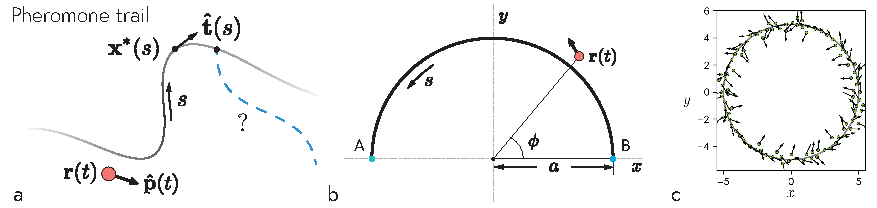
\includegraphics[width=\textwidth]{./figs/schematic.pdf}
    \label{fig:schm1}
    \caption{Schematic of setup}
\end{figure}

\subsection{Semi-circular trail}
For the problem at hand, we will considering a semi-circular trail whose coordinates can be
written in arc-length form as $\xst(s) = \{ a \cos(s/a), a \sin(s/a) \}$ where $a$ is the radius
of the circle. The trail starts at $s=0$ given by coordinates $\xst(0) = \{ a, 0 \}$ and ends at
$s=\pi a$ at $\xst (\pi a) = \{ -a, 0 \}$. From this it is easy to find that $\th(s) = \{ -\sin(s/a) , \cos(s/a) \}
= \{ \cos(\pi/2 + s/a), \sin(\pi/2 + s/a) \}$, and $\nh(s) = \{ -\cos(s/a) , \sin(s/a) \}$. We see that we
can represent $\th(s)$ through $\psi(s) = (\pi/2 + s/a)$. We can now calculate the location along the arc-length
where $\r(t)$ is closest by using the constraint condition $\d\r(t) \perp \th(s,t)$ or equivalently $\d\r(t)
\cdot \th(s,t) = 0$. We can now write $\d \r(t) \sim \{ a \cos(s/a) - r_x, a \sin(s/a) - r_y \}$
(up to normalization) and get the location $s_*(t) = a \tan^{-1}(r_y/r_x)$ by using the formula
for $\th(s)$. From this it is trivial to see that the angle along $\d \r$ is $\phi(t) = \tan^{-1}(r_y/r_x)$
(as is evident in Fig.~\ref{fig:schm1}$(b)$). For a given location of the agent, $\r(t)$ the orientation
it needs to take in the next step can be easily calculated to be $\theta(t) = (\pi/4 - \phi(t))$.

We can now set up the entire dynamics of the agent's trail following behavior on this semi-circle. We can state this
in the notation of reinforcement learning as it will become helpful later. The state of the agent
is $S^t = \{ r_x^t, r_y^t \}$, the measurements it makes are $M^t = \phi^t$ and using this information
the action the agent takes is $A^t = \{ \theta^t \}$ which is its orientation. The dynamics of
the agent can now be written as follows:
\begin{align}
    \text{Measurement update: } \phi^{t+1} = & \ \tan^{-1} \bigg( \frac{r_y^t}{r_x^t} \bigg) + \zeta^t, \\
    \text{Action update: }\ph^{t+1} =& \ \th^{t+1} + \d\r^{t+1}, \\
    \text{State update: } \r^{t+1} =& \ \r^t + l \ph^{t+1},
\end{align}
where $\r^t = \{ r_x^t, r_y^t \}$, $\d\r^t = (\xst(s^t)-\r^t)/||\xst(s^t)-\r(t)||$ and $\ph^t = \{ \cos \theta^t, \sin \theta^t \}$.
We have added sensory noise $\zeta^t$ (which is sampled from a uniform distribution) to the measurement
to reflect the error that accompanies measurements usually. The solution dynamics is shown
in Fig.~\ref{fig:schm1}$(c)$. We call this line-following behavior as a policy
$\pi_\ite(\r, \phi): $
which denotes the agent's innate behavior to follow pheromone trails.

\end{document}